\documentclass[14pt]{extreport}
\usepackage[utf8]{inputenc}
\usepackage[russian]{babel}
\usepackage[top=20pt,bottom=70pt,left=40pt,right=40pt]{geometry}
\usepackage{amssymb}
\usepackage{amsmath}
\usepackage{graphicx}
\usepackage[nottoc]{tocbibind}
\renewcommand*\rmdefault{cmr}

\begin{document}
	\begin{titlepage}
		\begin{center}  
			\large{Московский государственный университет имени М.В. Ломоносова\\
			Факультет вычислительной математики и кибернетики}\\
		\end{center}
		\begin{center}
			\vspace{160pt}
			\LARGE{\textbf{Формальные языки и автоматы\\}}
			\LARGE{\textbf{Методичка для сдающих и пересдающих}}
			\vspace{320pt}
		\end{center}
		\begin{center}
			\large{Может, зайдет кому-нибудь}
		\end{center}
	\end{titlepage}
	\newpage
	\tableofcontents
	\newpage
	\chapter*{Предисловие}
		Однажды я сдавал формалки. Не самый приятный опыт в моей жизни. Когда я ждал результатов,
		я сказал, что если не сдам, напишу методичку по этому чудесному предмету.\\
		\\
		Как несложно догадаться, я тогда не сдал.
		\\\\
		По формалкам уже есть отличное руководство в виде решений задач от Тани (не знаю, кто это,
		но если бы ее не было, статистика сдаваемости была бы гораздо хуже, я уверен, Таня,
		спасибо, что ты есть), и казалось
		бы - зачем я это делаю?\\
		Ну во-первых, я сказал, что напишу.\\
		Во-вторых, это довольно знатный способ подготовки к пересдаче, который потенциально
		поможет каким-нибудь людям после меня.\\
		В-третьих, наверное, есть смысл восполнить пробел в нормальном "печатном" пособии по
		формальным языкам. Ахо Ульмана я не читал (а он, может быть, и норм), но\ "Теорию
		Построения Комплияторов"\ читать совершенно невозможно.
		\\\\
		В этой методичке я в меру своих возможностей постараюсь не только подробно
		расписать решения различных задач (это уже есть у Тани), но и более-менее человеческим
		языком расписать, как применяемые алгоритмы работают (потому что выучить алгоритм, если
		есть примерное понимание работы, гораздо проще)
		\\\\
		За кривой русский язык извиняйте - я ЕГЭ сдал на 30 баллов.
	\newpage
	
	\chapter{Немного теормина}
	Недетерменированный конечный автомат - НКА
	\newpage
	
	\chapter{НКА по регулярному выражению}
	\section*{Алгоритм}
	Построение НКА по РВ делается по определенным правилам\\
	Каждое РВ можно разбить на подвыражения, а для простейших подвыражений автомат строится
	довольно просто\\
	На рисунке далее\\
	1. Е-переход\\
	2. Переход по символу $a$\\
	3. Переход по $a|b$ ($a$ или $b$)\\
	4. Переход по $ab$ (сначала $a$, потом $b$)\\
	5. Переход по $a*$ (сколько угодно символов $a$, в т.ч. 0)\\
	Справа от простейших НКА нарисованы общие НКА, когда переход совершается
	по некоторому РВ, где $r$ - РВ, а $M(r)$ - НКА, построенный по нему.\\
	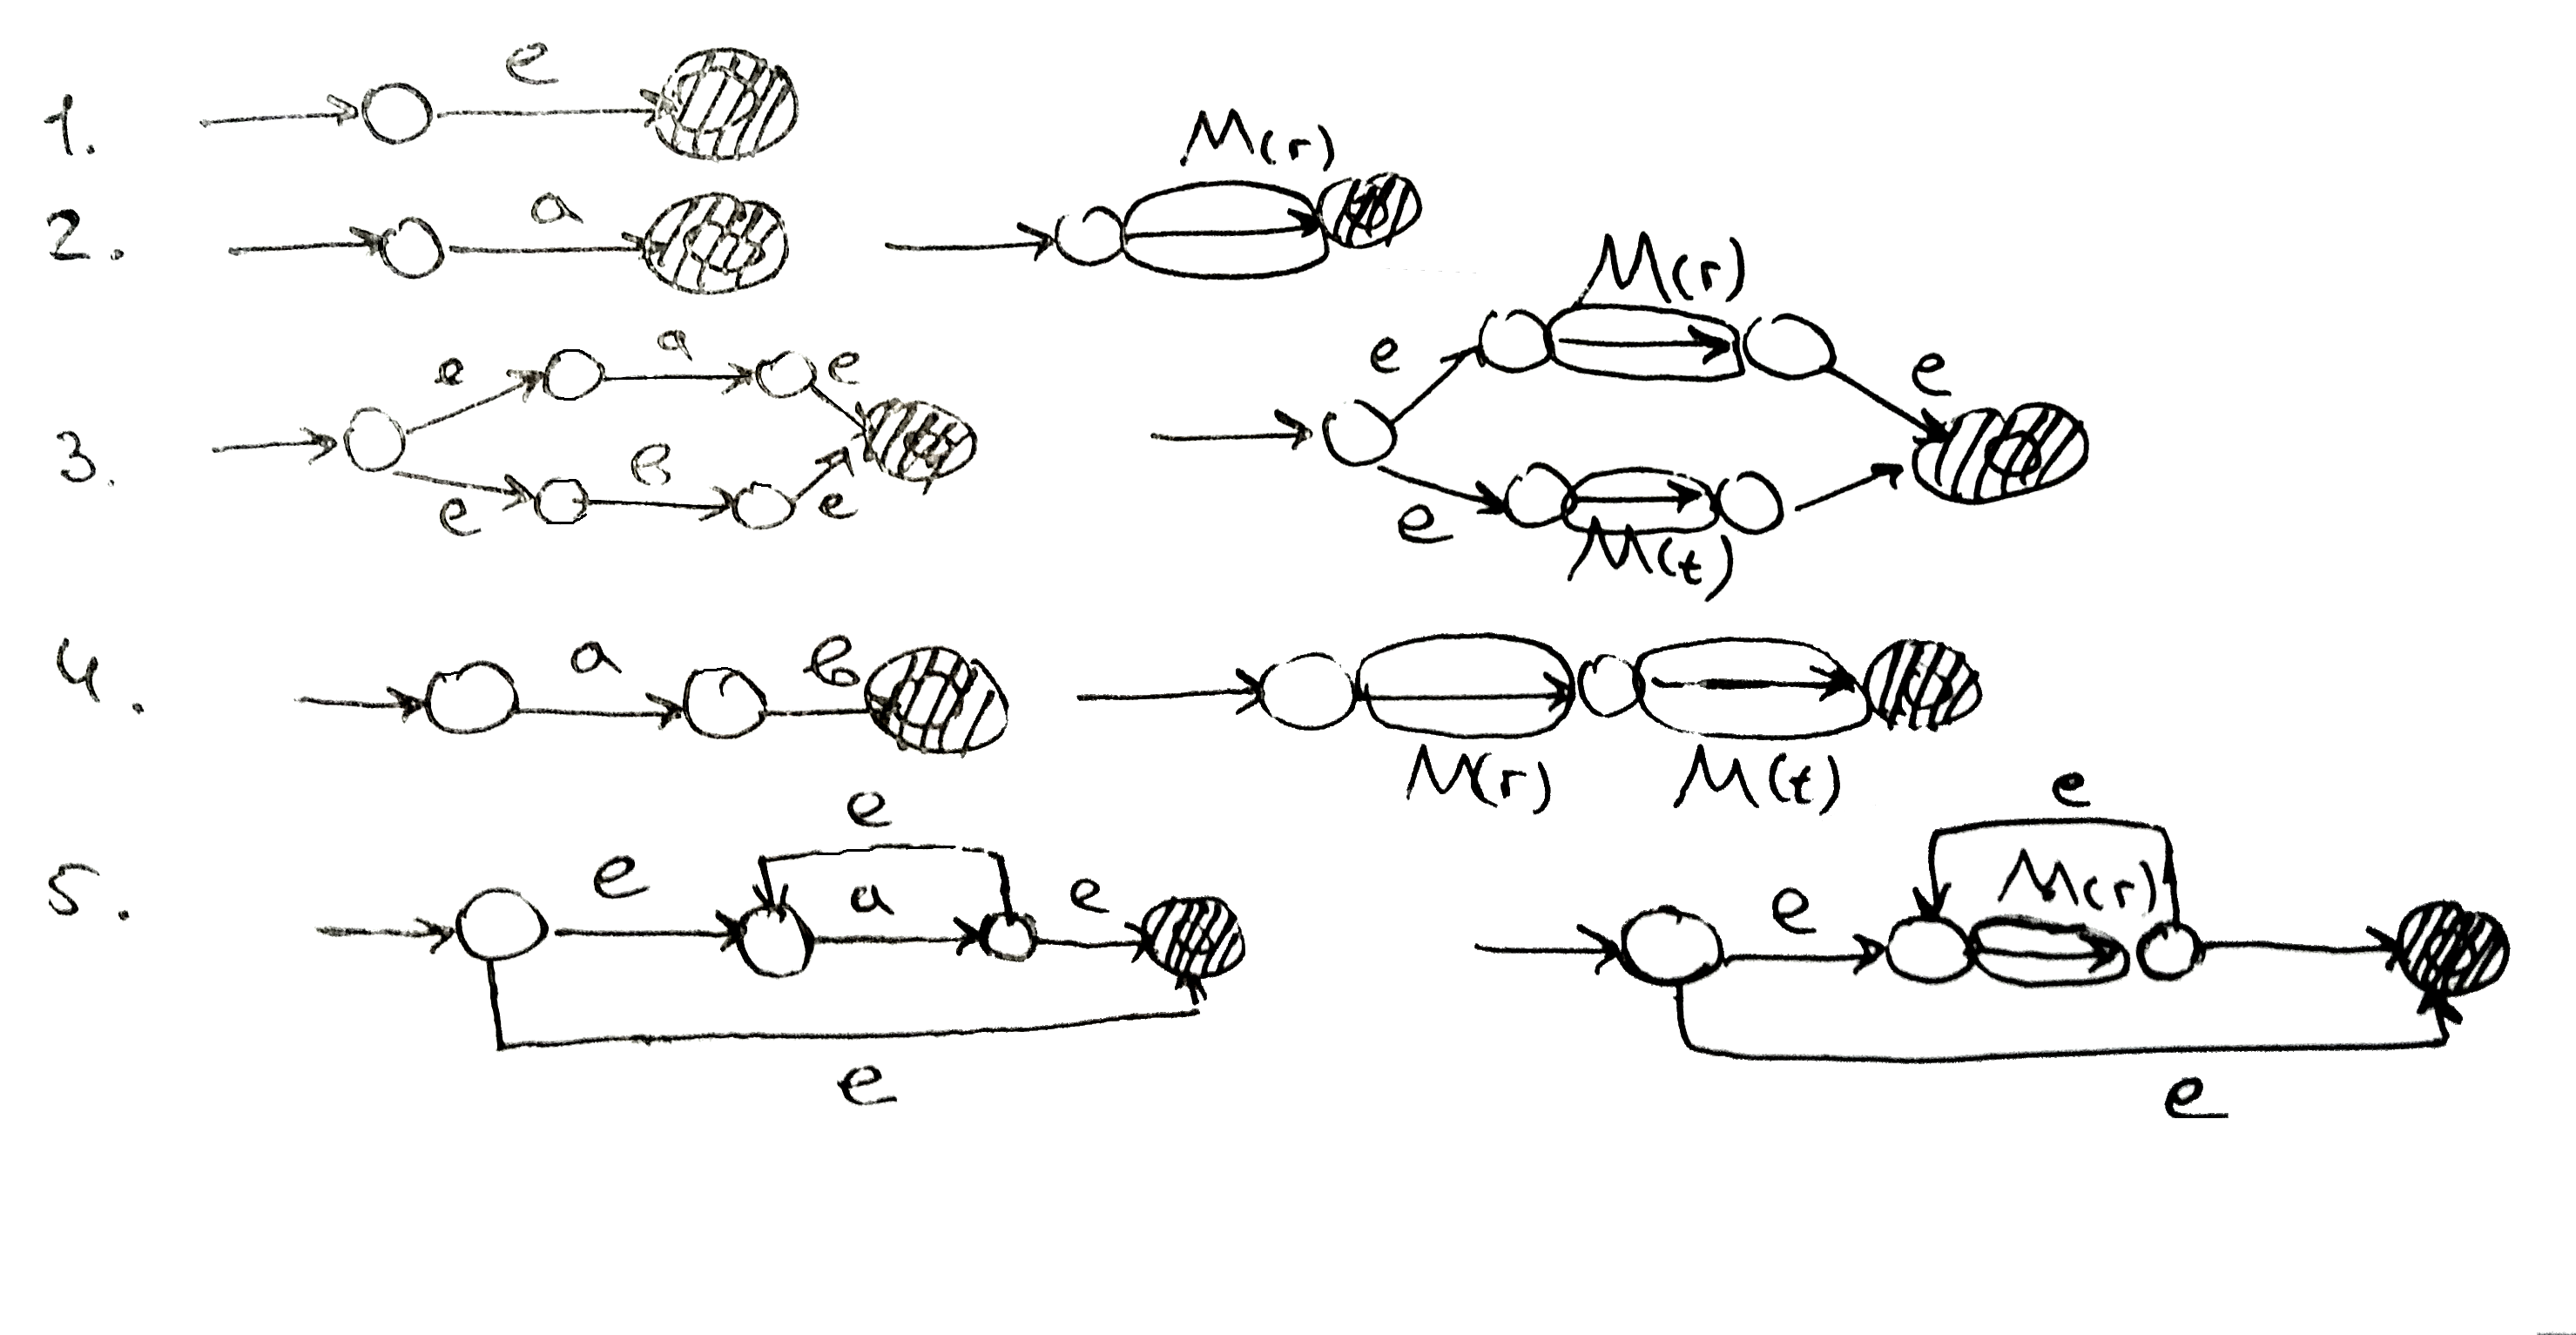
\includegraphics[scale=0.13]{data/pic1_1.png}\\\\\\\\
	На рисунке изображено построение НКА для РВ $b(a|ba)*|aab$\\
	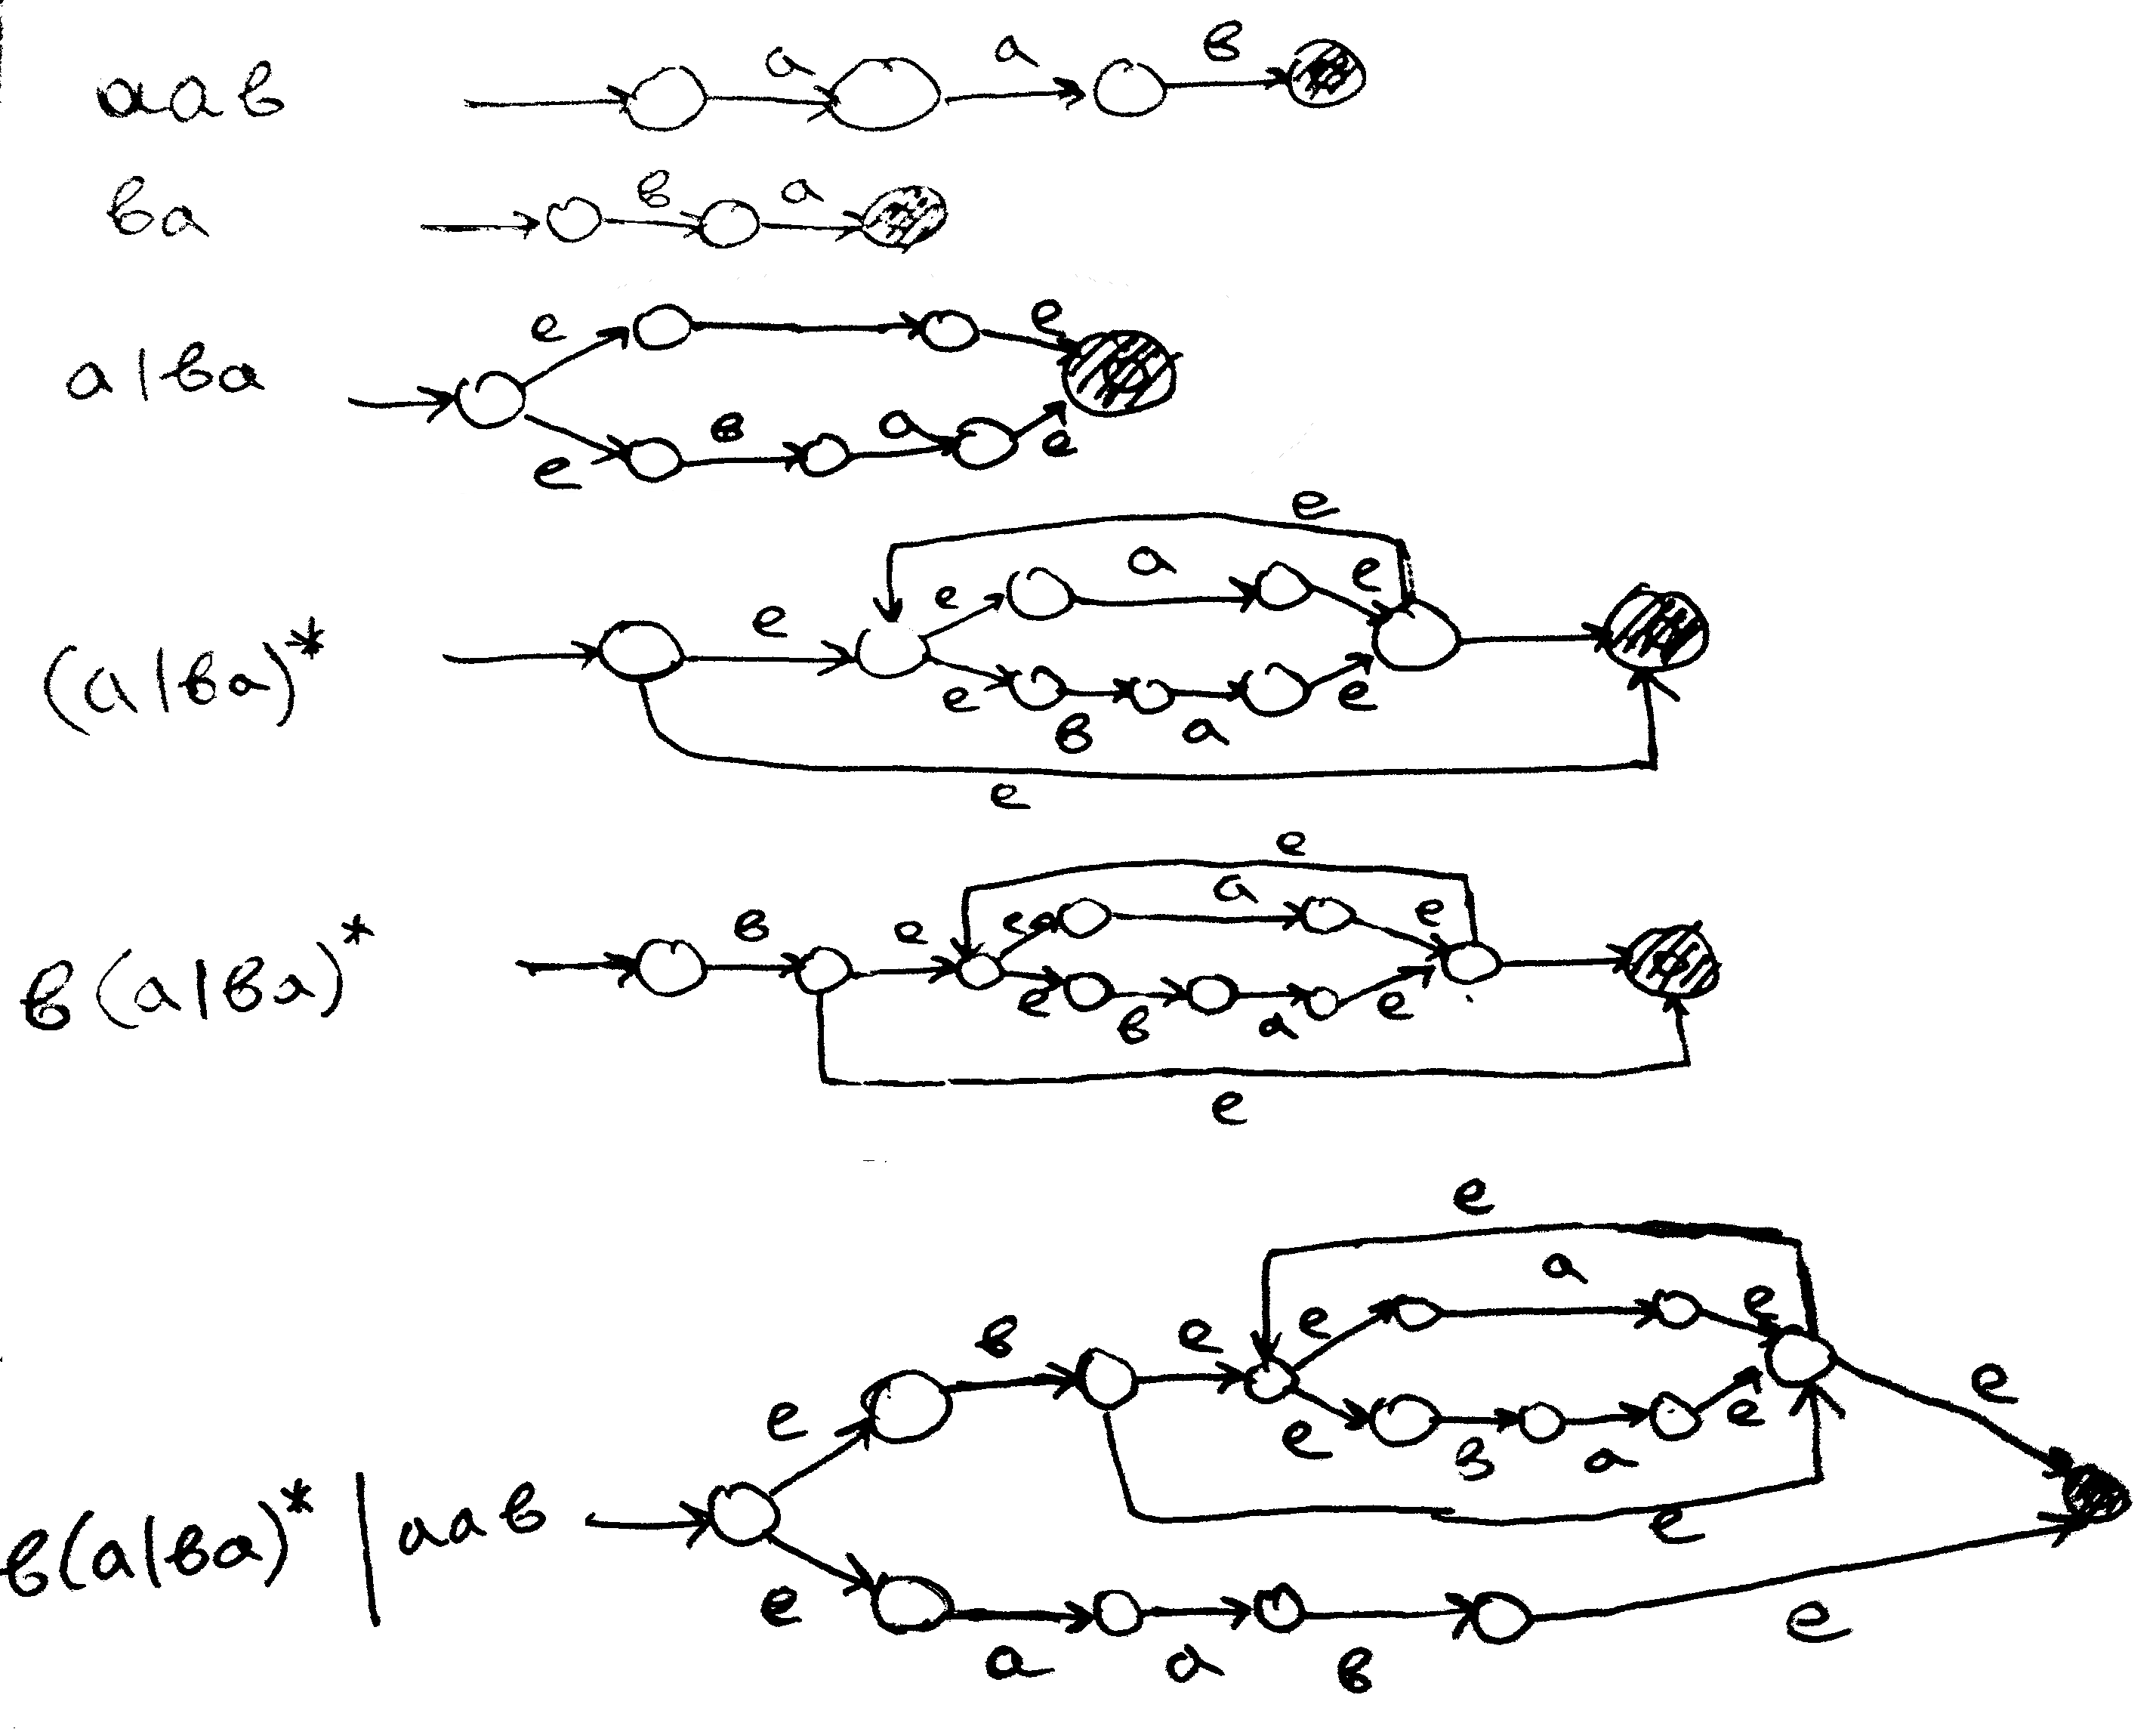
\includegraphics[scale=0.15]{data/pic1_2.png}\\
	\section*{Почему это работает}
	Правильность таких построений довольно очевидна, но если не верится, можно походить по
	полученным НКА по дугам и убедиться, что ничего кроме того, что описано в РВ, по ним
	составить нельзя.
	\newpage
	
	\chapter{ДКА по НКА}
	Глядя на НКА, полученные по РВ может показаться, что там слишком много лишних e-переходов,
	и они бесят. Также НКА это вам не ДКА: есть неопределенности которые бесят (хотя процесс
	детерминирования бесит больше). В любом случае существует алгоритм, позволяющий из большого,
	но красивого НКА получить маленький и очень некрасивый ДКА.
	\section*{Алгоритм}
	Введем некоторые обозначения:\\\\
	1. $e$-$closure(R)$ (эпсилон-замыкание состояния R) - множество состояний, в которые можно
	попасть из состояния $R$ по символу $e$. Стоит отметить, что "скачков"
	может быть больше одного,
	то есть, если в состояние $Q$ можно попасть из $P$ по $e$, а из $Q$ можно по $e$ попасть в $R$,
	то $R \in e$-$closure(Q)$. На языке умных людей это называется транзитивностью, но я тут не
	сложными словами щеголять пришел.\\\\
	2. $move(R, a)$ (достижимые из $R$ по $a$) - множество состояний, в которые можно попасть из
	состояния $R$ по символу $a$. (тут скачок должен быть только один)\\\\
	В качестве примера рассмотрим уродца из предыдущей главы: НКА по РВ\\ $b(a|ba)*|aab$
	\newpage
	1. Для начала все состояния надо пронумеровать\\
	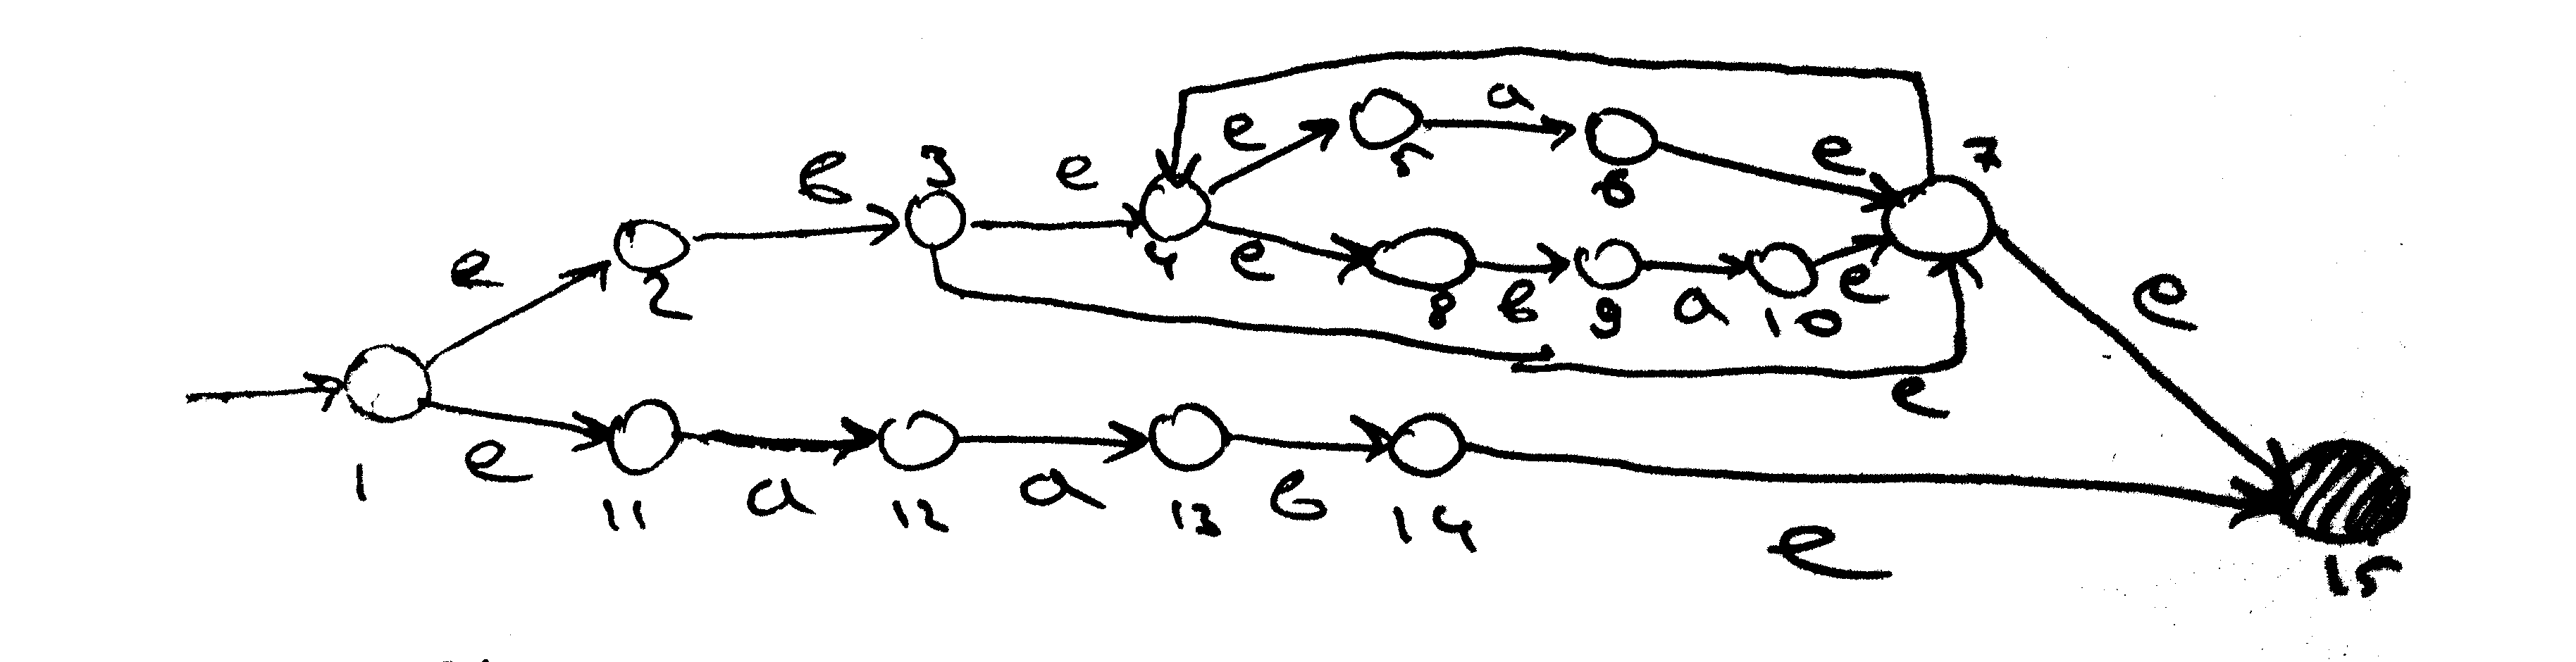
\includegraphics[scale=0.13]{data/pic2_1.png}\\
	На самом деле нумеровать их необязательно, главное дать им такие обозначения, чтобы
	вы сами могли отличить одно состояние от другого (ну и чтобы проверяющий экзаменатор не
	охерел, поэтому арабская вязь, наверное, не лучшее решение) - тут есть простор для фантазии,
	но на мой взгляд цифры вполне удобны (хотя между ними и приходится ставить запятые,
	если выписывать их в ряд).\\
	Далее мы начинаем описывать новый автомат с новыми состояниями - тут уже традиционно
	используют заглавные латинские буквы. Каждое новое состояние описывается множеством 
	старых состояний из первого автомата.\\
	2. В качестве начального состояния нового ДКА берут $A=e$-$closure(1)$, в нашем случае
	это $A=\{1, 2, 11\}$.\\
	3. Далее формируются следующие правила переходов:\\
	$D(A, a) = move(A, a)+e$-$closure(move(A, a))$\\
	$D(A, b) = move(A, b)+e$-$closure(move(A, b))$\\
	И т.д.\\
	Пусть вышло так, что есть состояние $Q$, из которого по символу $b$ мы переходим в состояние,
	описываемое множеством $\{1, 2, 3, 4, 6, 8, 12, 23\}$. При этом, если у такого множества уже
	есть имя, например $W$, то это попросту значит, что $D(Q, b)=W$. Если такого множества раньше
	не встречалось, то оно добавляется в таблицу состояний нового ДКА.\\
	Звучит сложно и скучно, поэтому лучше посмотреть на живой пример.\\
	$A=\{1, 2, 11\};$\\
	$move(A, a) = move(1, a)+move(2, a)+move(11,a);$\\
	$move(A,a)=\{\}+\{\}+\{12\}=\{12\};$\\
	$e$-$closure(move(A, a))=\{\};$\\
	$D(A, a) = move(A, a)+e$-$closure(move(A, a))=\{12\}+\{\}=\{12\};$\\
	Состояния $\{12\}$ у нас еще не было, поэтому добавим его в таблицу состояний и назовем его
	$B$.\\
	Проделаем аналогичные выкладки для символа $b$.\\
	$move(A, b) = move(1, b)+move(2, b)+move(11,b);$\\
	$move(A, b) = \{\}+\{3\}+\{\}=\{3\};$\\
	$e$-$closure(move(A, b))=\{4, 5, 7, 8, 15\};$\\
	$D(A, b) = move(A, b)+e$-$closure(move(A, b))=\{3\}+\{4, 5, 7, 8, 15\}=
	\{3, 4, 5, 7, 8, 15\};$\\
	Состояния $\{3, 4, 5, 7, 8, 15\}$ у нас тоже еще не было, поэтому запишем его в таблицу
	состояний ДКА.\\
	Подобные вычисления надо проводить для каждого символа в алфавите, для каждого нового
	состояния в таблице до тех пор, пока все старые состояния не будут описаны.\\
	С виду может показать, что это очень много писанины, но на деле все эти преобразования
	делаются в уме и единственное, что нужно реально выписывать, это таблицу состояний.\\
	Привожу финальную таблицу переходов для НКА из предыдущей главы.\\
		\begin{tabular}{lcc}
			 & $a$ & $b$ \\
			$A\{1, 2, 11\}$ & $B$ & $C$ \\
			$B\{12\}$ & $D$ & x \\
			$*C\{3, 4, 5, 7, 8, 15\}$ & $F$ & $G$ \\
			$D\{13\}$ & x & $E$ \\
			$*E\{14, 15\}$ & x & x \\
			$*F\{4, 5, 6, 7, 8, 15\}$ & $F$ & $G$ \\
			$G\{9\}$ & $H$ & x \\
			$*H\{4, 5, 7, 8, 10, 15\}$ & $F$ & $G$ \\	
		\end{tabular}\\\\
	Внимательный читатель заметит, что некоторые состояния отмечены звездочками и
	спросит, что это. Отвечаю: звездочками помечены конечные состояния. И это следующее
	правило алгоритма построения:\\
	4. Конечными состояниями нового ДКА помечаются такие состояния, которые содержат в себе
	конечное состояние старого НКА.\\
	В данном случае конечным состоянием является 15, поэтому все состояния, имеющие в себе
	15 становятся конечными.\\
	На рисунке изображен полученный ДКА.\\
	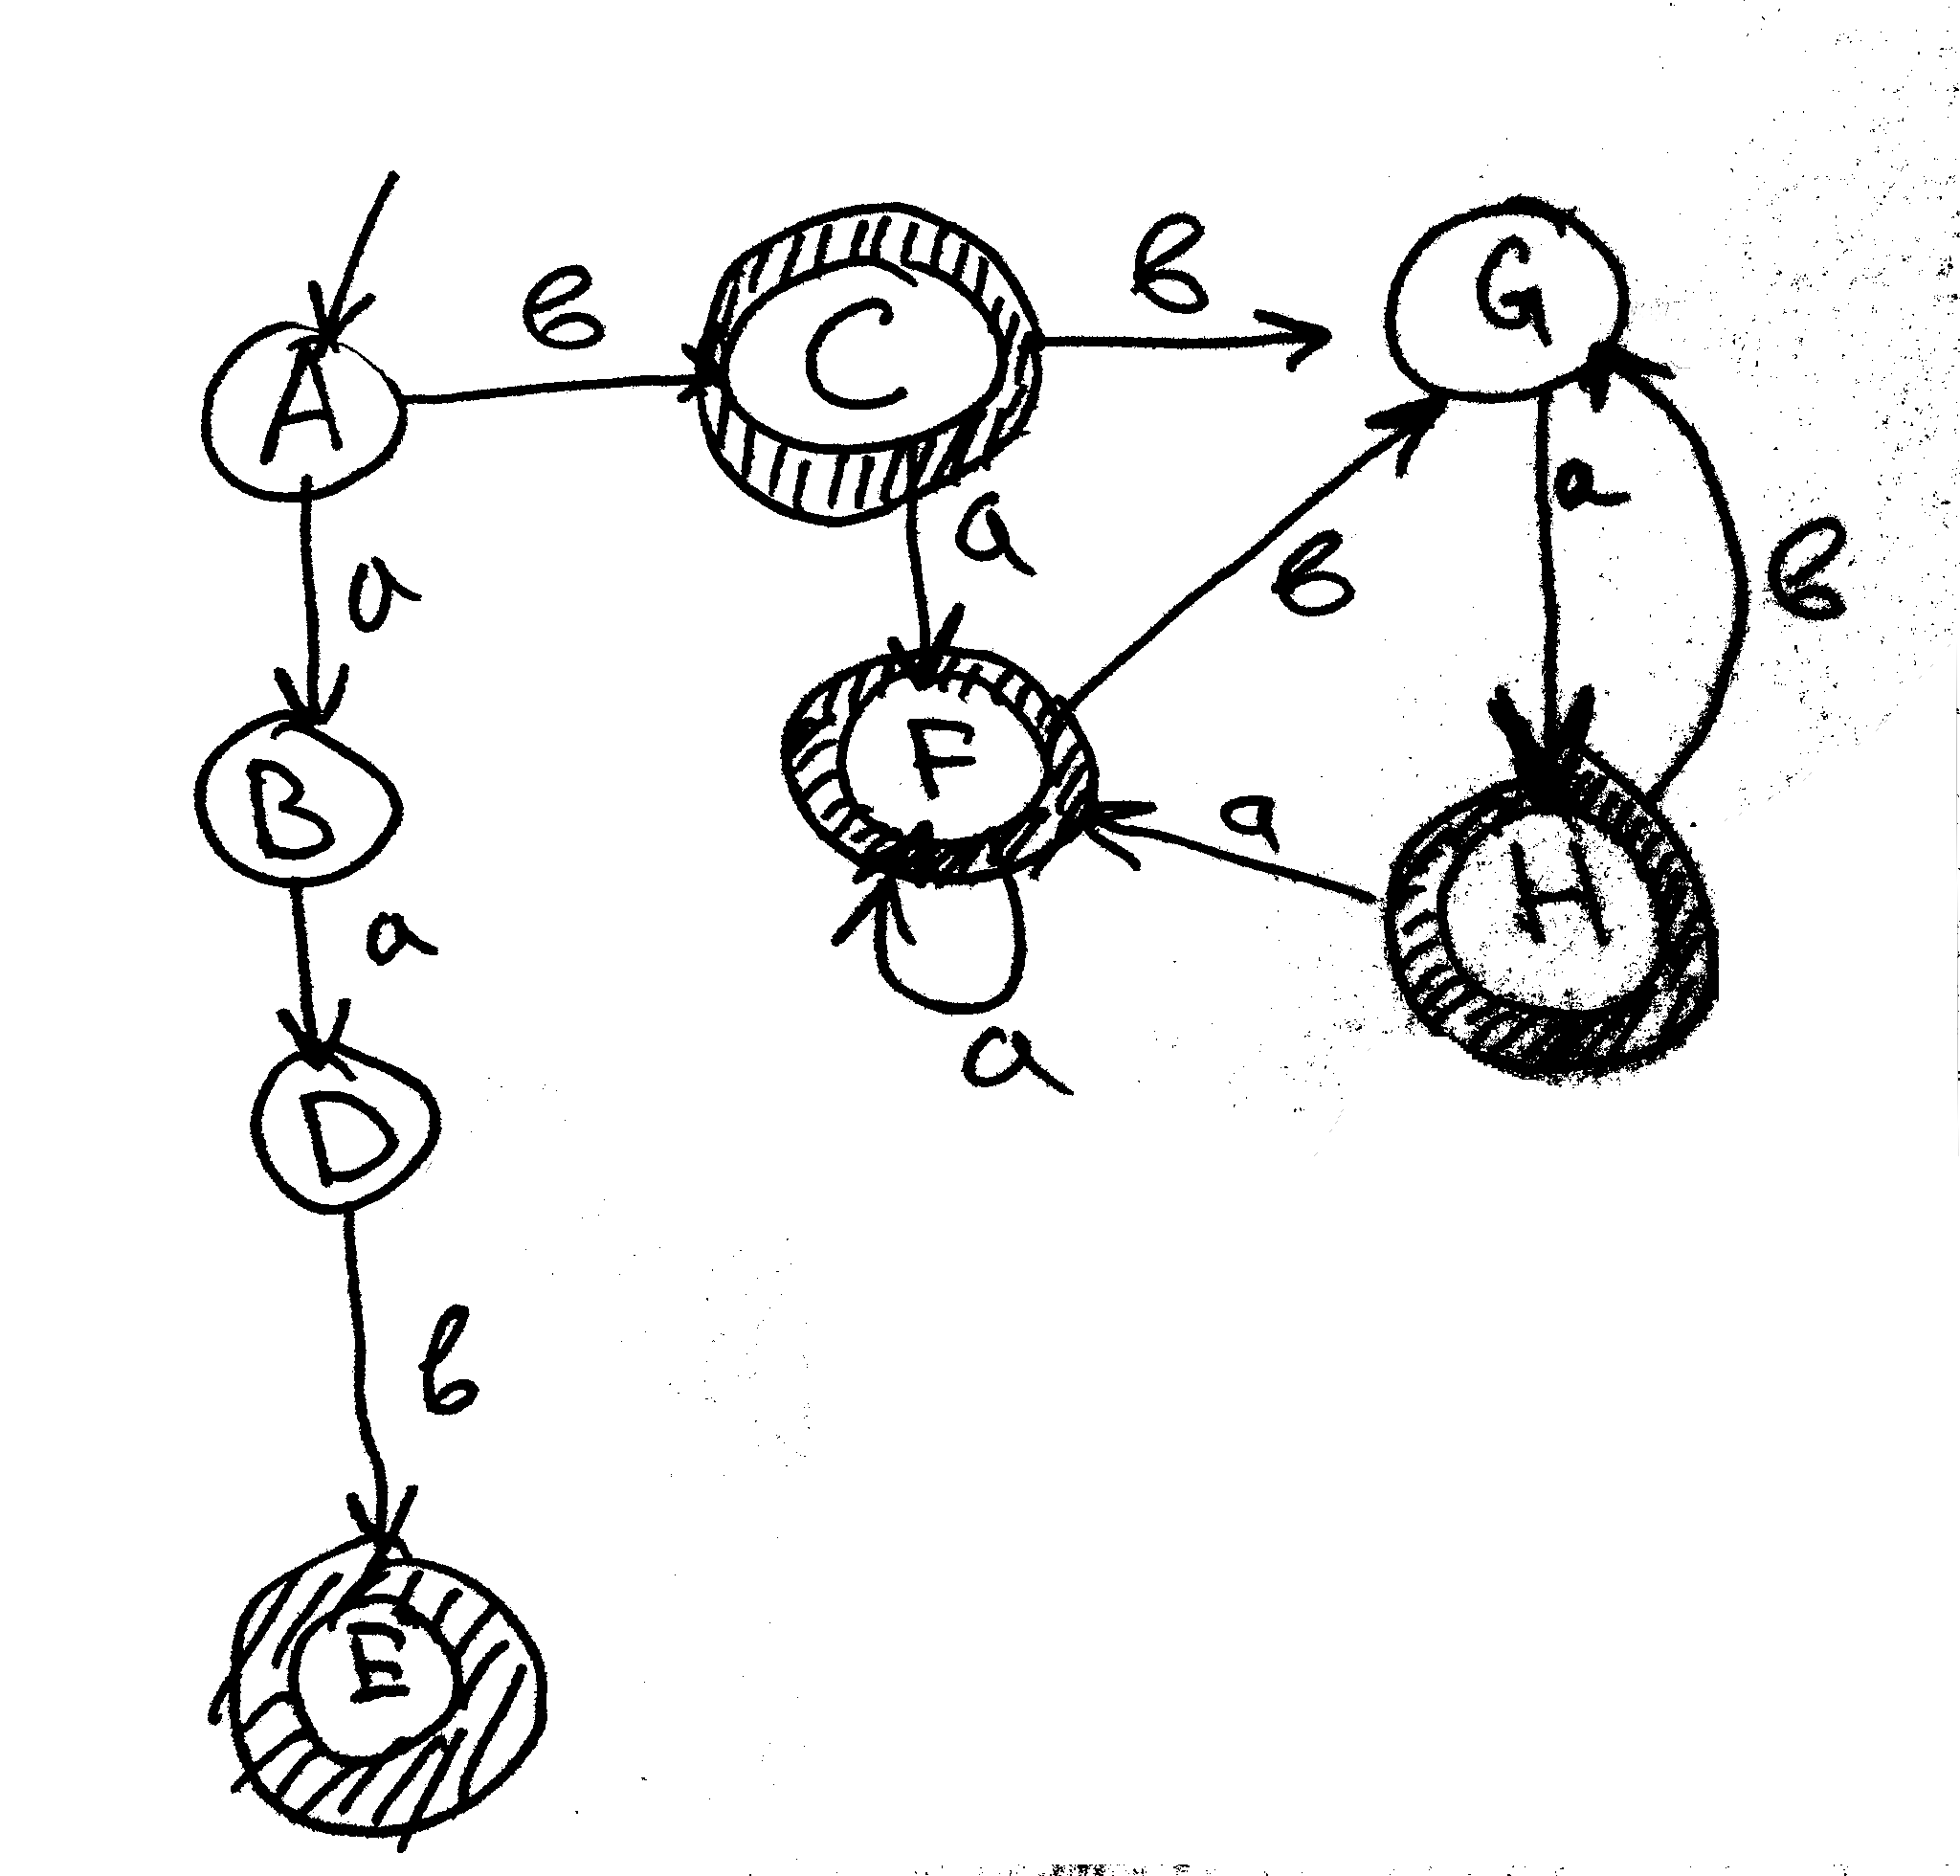
\includegraphics[scale=0.14]{data/pic2_2.png}\\
	\section*{Почему это работает}
	Работа алгоритма строится на двух мыслях:\\
	1. Если из одного состояния по $e$ можно перейти в несколько других,
	то зачем нам эти другие состояния, если по сути состояние одно, просто
	разибитое на несколько частей? (незачем)\\
	Грубо говоря, мы стягиваем за $e$-дуги много состояний в одно, как за веревки.\\
	2. Если после стягиваний состояний, две дуги, раньше шедшие в два разных состояния,
	теперь идут в одно стянутое, то действительно ли между этими дугами есть разница? (нет)\\
	
\end{document}
